\section{Temporal-Difference Learning}
Dieser Abschnitt behandelt das \ac{RL} Teilgebiet des \acl{TDL} (\ac{TDL}).
Zunächst wird das Konzept von \ac{TDL} am Beispiel von \ac{TD} Prediction erklärt. 
Anschließend werden die darauf basierenden \ac{TD} Algorihtmen \bothAlgs vorgestellt und miteinander verglichen.

\subsection{Temporal-Difference Prediction}
\label{sec:td_prediction}

Wenn ein \ac{RL} Problem als ein \ac{MDP} beschrieben werden kann, aber die State-Transition Probability oder die Rewardfunktion nicht bekannt sind, kann kein Modell der Umgebung erstellt werden. 
Folglich lassen sich diese \ac{RL} Probleme nicht mittels Dynamic Programming lösen. 
\ac{TDL} ist ein Teilgebiet von \ac{RL}, das Methoden definiert, die kein Modell der Umgebung und ihrer Dynamik benötigen. 
Stattdessen lernen \ac{TD} Methoden direkt durch Interaktion mit der Umgebung.
\ac{TDL} gilt daher als einer der zentralen Meilensteine von \ac{RL} und \ac{TD} Methoden werden als modellfreies RL bezeichnet \cite[S. 119]{suttonReinforcementLearningIntroduction2018}.
Die Voraussetzung zur Anwendung von \ac{TDL} ist, dass der Agent wie in \cref{formalisierung} beschrieben mit der Umgebung gemäß einer Policy $\pi$ interagieren kann \cite[S.88, S. 94]{kontesg.SeminarReinforcementLearning2021}. 

Von der Umgebung erhält der Agent seinen aktuellen Zustand $S_t$ und nach einer Aktion $A_t$ im nächsten Zeitschritt den Folgezustand $S_{t+1}$ und Reward $R_{t+1}$. 
Das Tupel $(S_t, A_t, S_{t+1}, R_{t+1})$ ist ein Sample (\dt Probe) von der Umgebung. 
Auf Basis der Samples schätzt \ac{TD} Prediction die zur Policy $\pi$ zugehörige State-Value Funktion $v_\pi$.
Der Schätzwert der State-Value-Funktion $V$ wird zu Beginn für jeden Zustand willkürlich initialisiert. \cite[S. 120f.]{suttonReinforcementLearningIntroduction2018}

Das Schätzen der State-Value Funktion durch Interaktion ist möglich aufgrund der in \cref{eq:statevalue_relation} definierten Beziehung zwischen State-Values aufeinander folgender Zeitschritte. 
Nach dieser Gleichung ist der exakte Wert der State-Value Funktion unter Policy $\pi$ eines Zustands $S_t$ der direkte Reward $R_{t+1}$ und der State-Value des Folgezustands $S_{t+1}$. \cite[S. 120f.]{suttonReinforcementLearningIntroduction2018}

\begin{equation}
    \equationentry{Beziehung zwischen State-Value Funktionen}
    v_{\pi}(S_t)= R_{t+1}+v_\pi(S_{t+1})
\end{equation}

Da in einem Sample der Zustand, Reward und Folgezustand enthalten sind, kann der State-Value für den Zustand $S_t$ auf Basis des darauffolgenden Zeitschritts geschätzt werden. 
Dieser Schätzwert für $V(S_t)$ wird als \ac{TD} Target bezeichnet. \cite[S. 120f.]{suttonReinforcementLearningIntroduction2018}

\begin{equation}
    \label{eq:td_target}
    \equationentry{Temporal-Difference Target}
    V(S_t)= R_{t+1}+\gamma V(S_{t+1})
\end{equation}

Da das \ac{TD} Target den Reward aus der Umgebung enthält, ist es ein besserer Schätzwert für $S_t$ als der willkürlich initialisierte Schätzwert $V(S_t)$. 
Die Differenz zwischen beiden Schätzwerten wird als \ac{TD} Error $\delta_t$ bezeichnet. 
Der \ac{TD} Error beschreibt den Unterschied zwischen zwischen dem alten und neuen Schätzwert und somit wie gut die alte Schätzung war. \cite[S. 120f.]{suttonReinforcementLearningIntroduction2018}

\begin{equation}
    \label{eq:td_error}
    \equationentry{Temporal-Difference Error}
    \delta_t = R_{t+1} + \gamma V(S_{t+1}) - V(S_t)
\end{equation}

Da das \ac{TD} Target ein besserer Schätzwert für $S_t$ ist, muss der Schätzwert $V(S_t)$ in Richtung des \ac{TD} Target korrigiert werden. 
Diese Aktualisierung ist das \ac{TD} Update und ein exponentiell geglätteter Mittelwert. \cite[S. 33]{suttonReinforcementLearningIntroduction2018}
\cref{eq:td_update} zeigt die Formel für das \ac{TD} Update. 
Im \ac{TD} Update wird der alte Schätzwert gemäß einer Lernrate $\alpha$ aktualisiert, die die Gewichtung des \ac{TD} Error festlegt. \cite[S. 120]{suttonReinforcementLearningIntroduction2018}

\begin{equation}
    \label{eq:td_update}
    \equationentry{Temporal-Difference Update}
    V(S_t) \leftarrow V(S_t) + \alpha [R_t+\gamma V(S_{t+1}) -V(S_t)]
\end{equation}

Um die State-Value Funktion für alle Zustände $S$ zu schätzen, interagiert der Agent wiederholt über mehrere Episoden mit der Umgebung. 
Nach jedem Zeitschritt führt der Agent für den im vorherigen Zeitschritten besuchten Zustand das \ac{TD} Update durch. 
Dieser Ablauf bildet die Grundlage für alle \ac{TD} Methoden. \cite[S. 121]{suttonReinforcementLearningIntroduction2018}
In \cite{suttonLearningPredictMethods1988} und \cite{watkinsQlearning1992} wurde bewiesen, dass \ac{TD} Prediction zur wirklichen State-Value Funktion $v_\pi$ konvergiert. 
Dafür müssen zwei Bedingungen erfüllt werden. 
Zum einen müssen alle Zustände hinreichend oft besucht werden. 
Zum anderen muss die im \ac{TD} Update genutzte Lernrate $\alpha$ hinreichend klein sein oder im Laufe des Trainings abnehmen. \cite[S. 33, S. 124]{suttonReinforcementLearningIntroduction2018}, \cite[S. 285 f.]{watkinsQlearning1992}

Am Beispiel von Gridworld aus \cref{sec:policy_statevalue} soll das \ac{TD} Update durchgeführt werden. 
Die Rewardfunktion und State-Transition Probability sind unverändert, dem Agenten jedoch nicht bekannt. 
In \cref{fig:gridworld_tdl} wird die zu untersuchende Policy dargestellt.
Die State-Values aller Zustände werden mit 0 initialisiert. 
Der blaue Pfeil zeigt die Zustandsübergänge des Agenten in der ersten Episode. 
Rechts neben der Abbildung ist das \ac{TD} Update mit Lernrate $\alpha=0,1$ und Diskontierungsfaktor $\gamma=0,9$ für den Zustand A3. 
Das \ac{TD} Update wird im darauf folgenden Zeitschritt durchgeführt und somit nachdem der Agent das Ziel A4 erreicht hat.

\begin{figure}
   \begin{minipage}[c]{.5\textwidth}
   \centering
    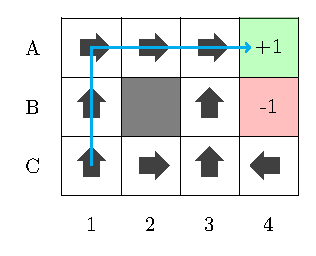
\includegraphics[]{gridworld/gridworld_tdl.pdf}
   \end{minipage}%
   \begin{minipage}[c]{.5\textwidth}
    $V(A3) \leftarrow V(A3)+ \alpha[R+\gamma V(A4)-V(A3)]\\
V(A3) = 0+0,1[-0,1+0,9 \cdot 1-0]=0,1$
   \end{minipage}
   \caption[\acs{TD} Update am Beispiel von Gridworld]{\acs{TD} Update am Beispiel von Gridworld. Der blaue Pfad zeigt den Pfad es Agenten in der ersten Episode. Rechts wird das \ac{TD} Update für den Zustand A3 berechnet. \protect\footnotemark}
   \label{fig:gridworld_tdl}
\end{figure}
\footnotetext{eigene Darstellung in Anlehnung an \cite[S. 99]{kontesg.SeminarReinforcementLearning2021}}